\chapter{\label{ch:2-zvp}The Zero Vector Potential Absorption Mechanism}

\minitoc

\section{Introduction}
Now is presented the Zero Vector Potential mechanism of attosecond absorption, proposed by \textit{Baeva et al} \cite{baeva_2006_TheoryHighorderHarmonic} and later developed by \textit{Savin et al} \cite{savin2017AttosecondscaleAbsorptionExtreme,savin2019EnergyAbsorptionLaserQED}. Laser energy absorption in dense plasmas was first proposed by Wilks and Kruer \cite{wilks1997}, a ponderomotive mechanism where plasma electrons are heated directly by the laser pulse via the so-called $\mathbf{J}\times \mathbf{B}$ force.

%At some point I should briefly chat about other absorption models (I think at the end of the intro - this will also include the stuff above. - Then I will start this chapter by talking about the case where JxB does not apply. ALso in the intro specify that for an overdense plasma, the laser does not propagate and must be reflected and hence we are generally talking about a laser-plasma surface interaction and the implications thereof.) Before this point I also want to discuss preplasmas.

This thesis focuses on the so-called `post-ponderomotive' regime where the frequency of the plasma oscillations ($\omega_p \sim \sqrt{n_e}$) are greater than the $\mathbf{J}\times \mathbf{B}$ induced plasma electron oscillations at $2\omega_L$. The plasma electrons are then fast enough to compensate the ponderomotive pressure of the laser pulse with the formation of electrostatic fields between electrons and ions and so respond adiabatically to the $\mathbf{J}\times \mathbf{B}$ force. Hence plasma electrons cannot be heated directly by the laser pulse. Note that this requires a sufficiently steep density gradient around the relativistic critical density surface (where $S=1$) to shift the main interaction to a region where this condition on the overdensity is satisfied. In this case the ponderomotive pressure of the laser compresses the electrons at the front surface of the plasma and so shifts the laser-plasma surface interaction to plasma densities well beyond the relativistic critical density, leaving behind a positive space charge. This electron-ion charge separation leads to the formation of a \textit{pseudo-capacitor} electrostatic field.


Interestingly working through the condition between $\omega_p$ and $\omega_L$ in normalised units suggests the criterion for this regime is $S > 4$, slightly more constraining than $S>1$ as is typically stated \cite{savin2019thesis}.

% at some point I must be explicitely clear about why this conditoin ad my sims with S=1 are compatible. This above criterion on S is associated with the bunch electrons. For S=1 we observe great compression of the target surface enabling us to enter the regime where the bunch S>4 whilst the bulk remains at S=1. Can thsi also be used to explain the energy absorption in phase one (bunch formation) ? Eneryg can be absorbed by JxB until the bunch density goes above some value???



[Come back to this and write up stuff about actaully it being the relativistc frequncy and critical density surfaces that matter and how this does indeed put a stricter condition on the bulk S value]

So we have entered a regime of adiabaticity where the plasma skin layer is confined within a potential well consisting of the ponderomotive pressure and the Coulomb potential. Consider a relativistic linearly polarised laser pulse obliquely incident, with an angle of incidence of $\theta$, on a semi-infinite plasma, existing for $x>0$. The Hamiltonian of a single electron confined within the potential well is
\begin{equation}\label{eq:hamiltonian_general}
	\mathcal{H} = c\sqrt{m^2_ec^2 + |\mathbf{p}|^2} + e\Phi.
\end{equation}
Here the first term is the electron energy, $U$, extracted from the invariant of the relativistic 4-momentum of the electron, $\mathbf{P^\mu} = (U/c, \mathbf{p})$,
\begin{equation}
	\mathbf{P^\mu \cdot P_\mu} = \frac{U^2}{c^2} - |\mathbf{p}|^2 = m^2c^2.
\end{equation}
Note that while there has been growing interest in the curvature of spacetime by relativistic lasers [cite edward here], for modern high power lasers this effect is small and not relevant for this thesis. Throughout the inner product of 4-vectors is defined with the Minkowski Metric. [find alex citation on pg 89 of thesis]

The second term of equation \ref{eq:hamiltonian_general} describes the contribution to the electron's energy from the electrostatic potential of the pseudo-capacitor. Decomposing the electron's 3-momentum into orthogonal components: $p_\mathrm{prop}$, along the laser propagation direction, $p_\mathrm{pol}$, along the polarisation axis of the laser pulse and $p_\perp$, perpendicular to both, two simplifications can be made. Firstly, by canonical conservation of transverse momentum, $p_\mathrm{pol} = eA$, where $A$ is the laser vector potential. Secondly, in the case of a $p$-polarised laser pulse (the known optimum for ZVP electron bunch generation), the forces at play confine the electron trajectory to the  $p_\mathrm{prop}$-$p_\mathrm{pol}$ plane and the interaction geometry is in essence \ac{2D}.

[include a diagram alluding to this?-it is basically since B is out of the plane and all other E fields are in the plane, also perhaps provide a foot not here to explain how incidentally this all provides a succinct explanation of why p is better?]

Explicitly, the Hamiltonian is now
\begin{equation}\label{eq:hamiltonian_specific}
	\mathcal{H} = c\sqrt{m^2_ec^2 + p^2_\mathrm{prop} + e^2A^2} + e\Phi.
\end{equation}
From equation \ref{eq:hamiltonian_specific} it is clear that should the vector potential pass through zero, one of the walls of the potential well is suppressed, allowing electrons in the in the skin layer to escape the plasma, breaking adiabaticity. The necessity of vector potential zeros for this violent reconstruction of the plasma surface led Baeva et al \cite{baeva2011ZeroVectorPotential} to coin the term `Zero Vector Potential' mechanism to describe this process. Indeed, while in standard calculations a laser pulse will exponentially decay within a skin layer without passing through zero, Baeva et al \cite{baeva2011ZeroVectorPotential} were able to demonstrate in \ac{PIC} simulations that for this regime, zeros are able to propagate through the skin layer of the plasma. The explanation for this difference in mechanics relies on a Doppler shift in the laser field due to the relativistic motion of the ablating plasma surface, and the mathematical formalism of this process proceeds as follows.

[I think before this point it would be good to enter in the language of electron bunches or sheaths - I will continue the dicussion assuming this concept has been introduced].

As the \ac{ZVP} mechanism is a relativistic phenomenon, it is essential to consider the laser pulse propagating through a relativistically ablating electron bunch (i.e. with some component of its velocity anti-parallel to the laser pulse propagation direction). Transforming to the rest frame of the ablating front, beyond the relativistic critical density surface, the vector potential of the laser pulse will be an evanescent wave, at the spatial centre of the laser pulse, it can be described simply by
\begin{equation}
	\mathbf{A}'_\mathrm{L}(t',r') = A'_0\cos(\omega'_\mathrm{L}t')\exp(-r'/\delta')\hat{\mathbf{r}}'_\mathrm{pol}= A'_\mathrm{L}\hat{\mathbf{r}}'_\mathrm{pol},
\end{equation}
where the primed symbols indicate that these quantities are measured in the rest frame of the expanding front, $A'_0$ is the vector potential amplitude and $\omega'_\mathrm{L}$ is the frequency of the laser pulse, $r'$ is the propagation distance of the laser into the plasma, $\delta'$ is the skin depth and $\hat{\mathbf{r}}'_\mathrm{pol}$ a unit vector defining the polarisation direction of the laser pulse. Un-primed coordinates will indicate the lab frame measurements.

[For sure include a diagram of this]

While in previous demonstrations of the vector potential zeros, it was assumed that the ablation occurs normal to plasma surface, it is now known that this ablation occurs in the specular reflection direction and it is necessary to confirm that zeros are still predicted. Consider a p-polarised laser pulse confined to the $x$-$y$ plane incident with an angle of incidence $\theta$ on an ablating overdense plasma expanding with velocity $-v_f\hat{\mathbf{x}}$ in the lab frame, as in figure \ref{fig:zvp_ablatingfront}.
% TODO: \usepackage{graphicx} required
\begin{figure}
	\centering
	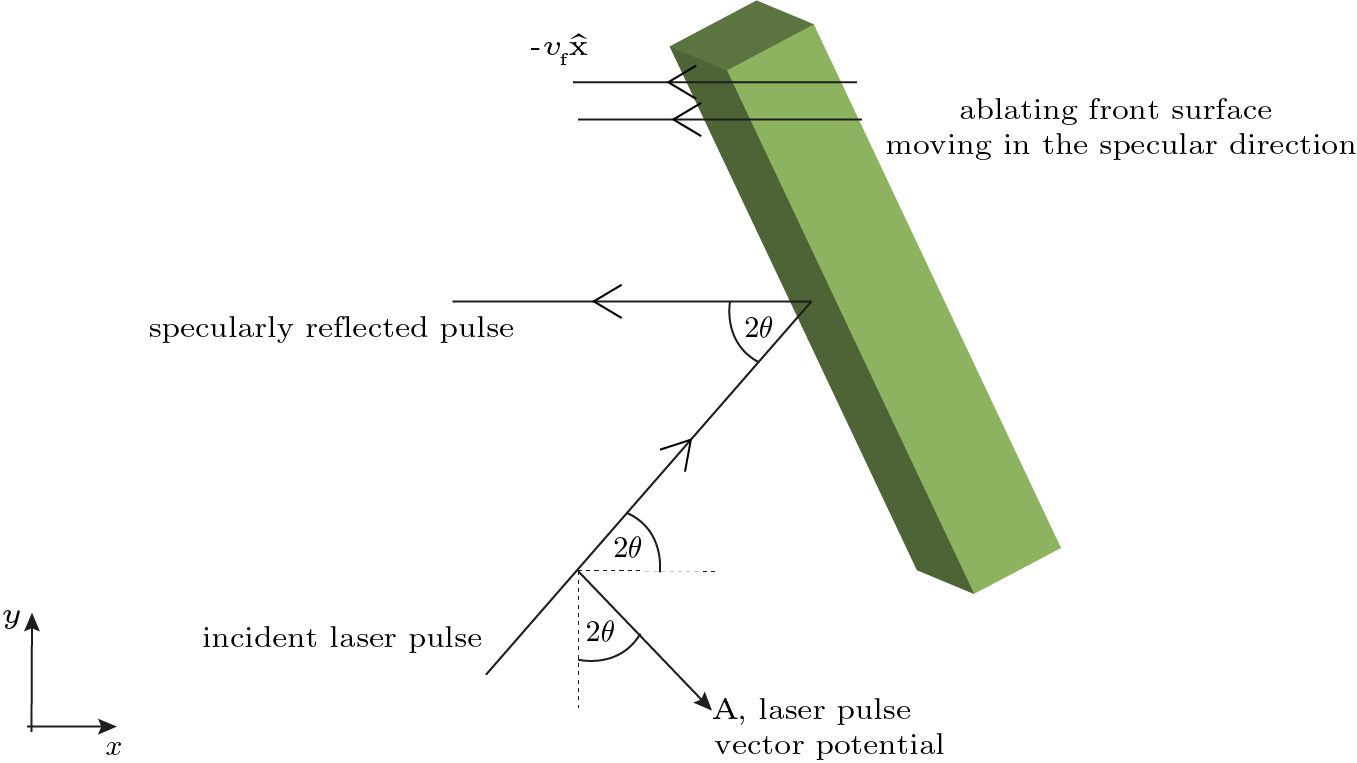
\includegraphics[width=0.7\linewidth]{../diagrams/zvp_ablating_front}
	\caption{Diagram of a $p$-polarised laser pulse incident on an ablating overdense plasma. The laser is incident obliquely at an angle of $\theta$ and is reflected specularly. The plasma ablates specularly also. The interaction geometry is confined to a 2D plane.}
	\label{fig:zvp_ablatingfront}
\end{figure}
The direction of polarisation is
\begin{equation}
	\hat{\mathbf{r}}_\mathrm{pol} = \hat{\mathbf{x}}\sin{2\theta} - \hat{\mathbf{y}}\cos{2\theta}
\end{equation}
and the velocity of the rest frame of the ablating front relative to the lab frame is $-v_f\hat{\mathbf{x}}$.

Applying the Lorentz transformation to the electromagnetic 4-potential,
\begin{equation}
	\mathbf{A}_\mu = (\phi/c,\mathbf{A}),
\end{equation}
explicitly,
\begin{equation}
	\mathbf{A}'_\mu = \Lambda^\mu_\nu \mathbf{A}'_\nu,
\end{equation}
where $\Lambda^\mu_\nu$, the Lorentz transform in this geometry is
\begin{equation}
	\Lambda^\mu_\nu = \begin{pmatrix}
			\gamma & -\beta\gamma & 0 & 0\\
			-\beta\gamma & \gamma & 0 & 0\\
			0 & 0& 1 & 0\\
			0 & 0 & 0 & 1
	\end{pmatrix}
\end{equation}
and here $\beta = -v_\mathrm{f}/c$, $\gamma = 1/\sqrt{1-\beta^2}$. Immediately from the $y$-coordinate transformation,
\begin{equation}\label{eq:zvp_lorentz_y}
	A'_\mathrm{L}\cos{2\theta'} = A_\mathrm{L}\cos{2\theta}.
\end{equation}
Applying the headlight effect for a source moving at an angle $2\theta$ to the boosted frame,

[I still need to include the headlight effect derivation]
\begin{equation}
	\cos{(2\theta')} = \frac{\cos{(2\theta)}-\beta}{1 - \beta\cos{(2\theta)}}
\end{equation}
and rearranging equation \ref{eq:zvp_lorentz_y}, the vector potential in the lab frame is
\begin{equation}\label{eq:zvp_labA}
	A_\mathrm{L} = \frac{1-\beta \sec{(2\theta)}}{1 - \beta\cos{(2\theta)}} A'_0\cos{(\omega'_L t')}\exp{(-r'/\delta')}.
\end{equation}
Writing the boosted frame space-time coordinates in terms of the lab frame coordinates,
\begin{equation}
	ct' = \gamma(ct-\beta x),
\end{equation}
\begin{equation}
	x' = \gamma(x-\beta ct),
\end{equation}
yields
\begin{equation}\label{eq:zvp_labAfull}
	A_\mathrm{L} =  A_0\cos{(\omega_L t - kx)}\exp{\left(-\frac{\sqrt{(x-\beta ct)^2+(y/\gamma)^2}}{\delta}\right)},
\end{equation}
where
\begin{equation}
	A_0 = \frac{1-\beta \sec{(2\theta)}}{1 - \beta\cos{(2\theta)}}A'_0,
\end{equation}
\begin{equation}
	\omega_L = \gamma \omega'_L,
\end{equation}
\begin{equation}
	k = \frac{\beta \gamma\omega'_L}{c},
\end{equation}
\begin{equation}
	\delta = \frac{\delta'}{\gamma}.
\end{equation}
The oscillatory term in equation \ref{eq:zvp_labAfull} demonstrates the propagation of vector potential zeros within the plasma target. From the structure of this term it would appear that these zeros are expelled from the plasma along the specular direction at a speed (recall beta is negative - change this earlier in the theory so that that negative sign is more explicit in the result.)
\begin{equation}
	v_\phi = \frac{\omega_L}{k} = \frac{c}{\beta} = -\frac{c^2}{v_\mathrm{f}}.
\end{equation}
Could also discuss here about how relativistic similarity theory derives that zeros move at speed c but how that cannot be valid since then we would always have infinitely thin radiation pulses, unless there is an extended range of zero? I suppose there is some radiation happening around the peak? Good questions..
One remaining consideration is we require that the zero gets through the whole electron bunch which is generally at very high density but is also very thin, in a way is this skin depth not what precisely determines the bunch width? The bunch will be compressed until the skin depth goes to zero across it perhaps? Things to think about.




